\documentclass[a4paper]{report}

\usepackage[utf8]{inputenc}
\usepackage[english]{babel}
\usepackage[T1]{fontenc}
\usepackage{textcomp}
\usepackage[]{amsthm} 
\usepackage[]{amssymb}
\usepackage{graphicx}
\usepackage{float}
\usepackage{soul}
\usepackage{color}
\usepackage{bm}
\usepackage{listings}
\usepackage{xcolor}
\usepackage{enumitem}
%\usepackage{xfrac}
\usepackage[normalem]{ulem}

% ~~~~ fancy symbol ~~~~
\usepackage{bbding}

% ~~~~ no indent per paragraph ~~~~-
\usepackage[parfill]{parskip}

% ~~~~ hyperlinks ~~~~ 
\usepackage[colorlinks=true, linkcolor=blue]{hyperref}

% ~~~~ subfigs ~~~~
\usepackage{subcaption}

% ~~~~ math ~~~~
\usepackage{amsmath}

\usepackage{mathtools}
% ~~ colorbox : "align" use only ~~
\newcommand{\myboxA}[1]{
	\fcolorbox{black}{lime}{#1}
}
\MakeAboxedCommand\AboxedA\myboxA

% ~~ colorbox : else ~~
\newcommand{\mybox}[1]{
	\fcolorbox{black}{lime}{$\displaystyle#1$}
}

% ~~~~ graphics ~~~~
\usepackage{tikz}
\usetikzlibrary{trees}
\usetikzlibrary {fit,shapes.geometric} % W: Command terminated with space. (1)
\usetikzlibrary {automata} % W: Command terminated with space. (1)
\usetikzlibrary{arrows.meta}
\usepackage{multicol}

\usepackage{pgfplots}
\pgfplotsset{compat = newest}

\usepackage{geometry}
\geometry{legalpaper, margin=1in}

% ~~~~ upgraded tables ~~~~
\usepackage{booktabs}

% ~~~~ algorithm formatting ~~~~
\usepackage{algorithm}
\usepackage[noend]{algpseudocode}
\usepackage{caption}

% ~~~~ list bullets ~~~~
\renewcommand{\labelitemii}{$\circ$}
\renewcommand{\labelitemiii}{$\star$}
\renewcommand{\labelitemiv}{$>$}

% figure support
\usepackage{import}
\usepackage{xifthen}
\pdfminorversion=7
\usepackage{pdfpages}
\usepackage{transparent}
\newcommand{\incfig}[1]{%
    \def\svgwidth{\columnwidth}
    \import{./figures/}{#1.pdf_tex}}

% Newline for algorithm psuedo
\newcommand{\algrule}[1][.2pt]{\par\vskip.5\baselineskip\hrule height #1\par\vskip.5\baselineskip}

% -------- Listings/XColor Settings --------
\definecolor{codegreen}{rgb}{0,0.6,0}
\definecolor{codegray}{rgb}{0.5,0.5,0.5}
\definecolor{codepurple}{rgb}{0.58,0,0.82}
\definecolor{backcolour}{rgb}{0.95,0.95,0.92}

\lstdefinestyle{mystyle}{
	backgroundcolor=\color{backcolour},
	commentstyle=\color{codegreen},
	keywordstyle=\color{magenta},
	numberstyle=\tiny\color{codegray},
	stringstyle=\color{codepurple},
	basicstyle=\ttfamily\scriptsize,
	breakatwhitespace=false,
	breaklines=true,
	captionpos=b,
	keepspaces=true,
	numbers=left,
	numbersep=5pt,
	showspaces=false,
	showstringspaces=false,
	showtabs=false,
	tabsize=4
}

\lstset{style=mystyle}

% -------------- Doc Start -------------------



\pdfsuppresswarningpagegroup=1

\title{\Huge{Designing a Fibonacci Accelerator}}
\author{\textbf{Authors:} \\WhisperingRock}
\date{Class\\CPE490: Open-Source ASIC Design\\\today}

\begin{document}
    \maketitle
	
	% ~~~~ add toc as a bookmark ~~~~
	\phantomsection
	\addcontentsline{toc}{section}{\contentsname}

	\tableofcontents

	\chapter{Introductions}
		In this lab, the task was to create a Fibonacci accelerator. Before
		going further in the paper, I must first describe the Fibonacci 
		sequence and what makes a design an \textit{accelerator}. 

		First, let's discuss the Fibonacci sequence using a recursive formula. 
		\[
			\bm{F_{n+2} = F_{n+1} + F_{n} \text{ where } F_0 = 0 \text{ and } F_1 = 1}
		\]

		In our discussion in class, another relationship emerged when comparing multiple terms.

		Consider:
		\begin{itemize}
			\item Let $F_{n} = a$ 
			\item Let $F_{n+1} = b$ 
			\item $F_{n+2} = a + b$
			\item $F_{n+3} = a + 2b$
			\item $F_{n+4} = 2a + 3b$
			\item $F_{n+5} = 3a + 5b$
		\end{itemize}

		If given two terms of the sequence, we can potentially calculate
		the next four terms from the initial two. This unique way to describe terms 
		has potential for a speed-up if we can utilize shifters and adders
		with the motivation to calculate many terms in a single cycle. 

		This motivation to increase throughput or performance over a CPU, 
		through the use of configurable logic, is termed as an \textit{accelerator}. 
		For this lab, our accelerator will calculate more than one term
		of the Fibonacci sequence per clock cycle. 

		Lastly, another motivation of this lab is to become familiar with 
		open-source tooling set. 

	\chapter{Procedure}
		The workflow of this lab, which is largely focused on design before
		synthesis, will be the following

		\begin{enumerate}
			\item LINTing based off of many tools s.a. Verilator, Icarus, GL, \ldots
			\item Simulation of test scripts on Verilator, then Icarus Verilog
			\item BMC verification 
			\item \textit{K}-Induction formal verification (optional)
		\end{enumerate}

	\chapter{Design}

		\begin{figure}[H]
			\centering
			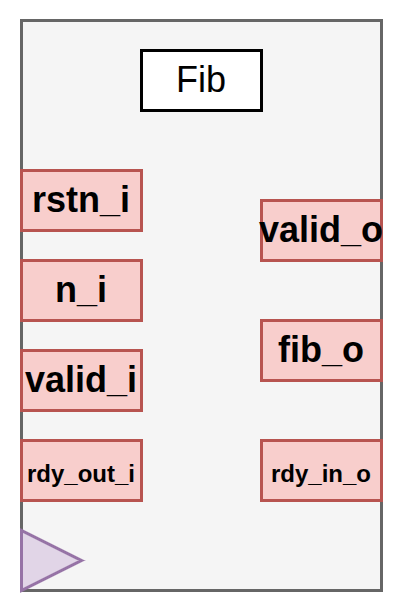
\includegraphics[
				width			= 0.3\textwidth,
				keepaspectratio	= true
			]{./pics/top.png}
			\label{fig:top}
			\caption{Fibonacci Top Module}
		\end{figure}

		The top-level module has a data and control signals:
		\begin{itemize}
			\item \textbf{clk\_i}: clock (posedge is captured).
			\item \textbf{rstn\_i}: active-low synchronous reset.
			\item \textbf{valid\_i}: indicates when input n\_i can be read.
			\item \textbf{n\_i}: requested term of fib sequence.
			\item \textbf{rdy\_out\_i}: indicates when downstream has read this modules output
				(and module can begin processing a new sequence).\\
			\item \textbf{valid\_o}: indicates module's output is ready to be read.
			\item \textbf{rdy\_on\_o}: indicates module is ready for a new request (n\_i).
			\item \textbf{fib\_o}: modules output ($F_{n}$).
		\end{itemize}


		In order to capture the functionality of these top-level signals, 
		an FSM was used:

		\begin{figure}[H]
			\centering
			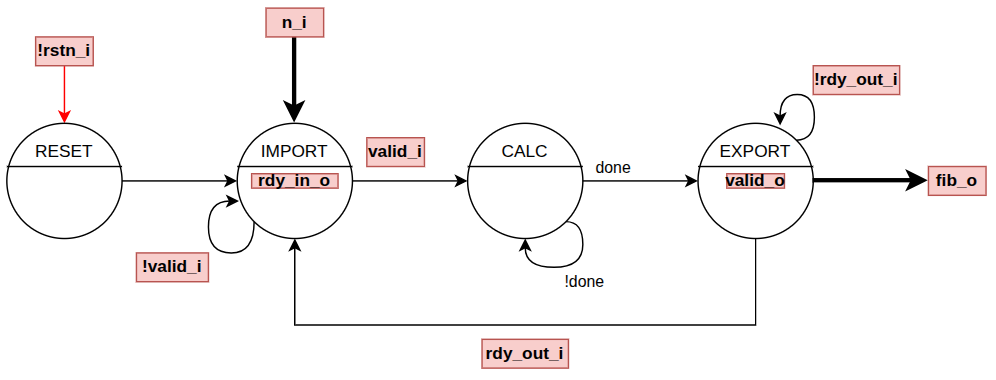
\includegraphics[
				width			= 0.8\textwidth,
				keepaspectratio	= true
			]{./pics/fsm.png}
			\caption{FSM of Fibonacci Accelerator}
			\label{fig:fsm}
		\end{figure}

		From here, lets take a closer look into the CALC stage of the FSM, where most
		of our accelerator logic comes into play. An attentive reader will notice that there 
		are only two adders and a single shifter: there is a considerable 
		amount of adders required to further calculate $F_{n+4}$ and $F_{n+5}$.
		Since this must be implemented in ASIC where wires and hardware are not
		free lunches, this designer opted to take 2 cycles to calculate 4 terms 
		of the fib sequence. This will keep the area smaller while producing
		two elements per cycle (a +2x increase over a CPU).

		\begin{figure}[H]
			\centering
			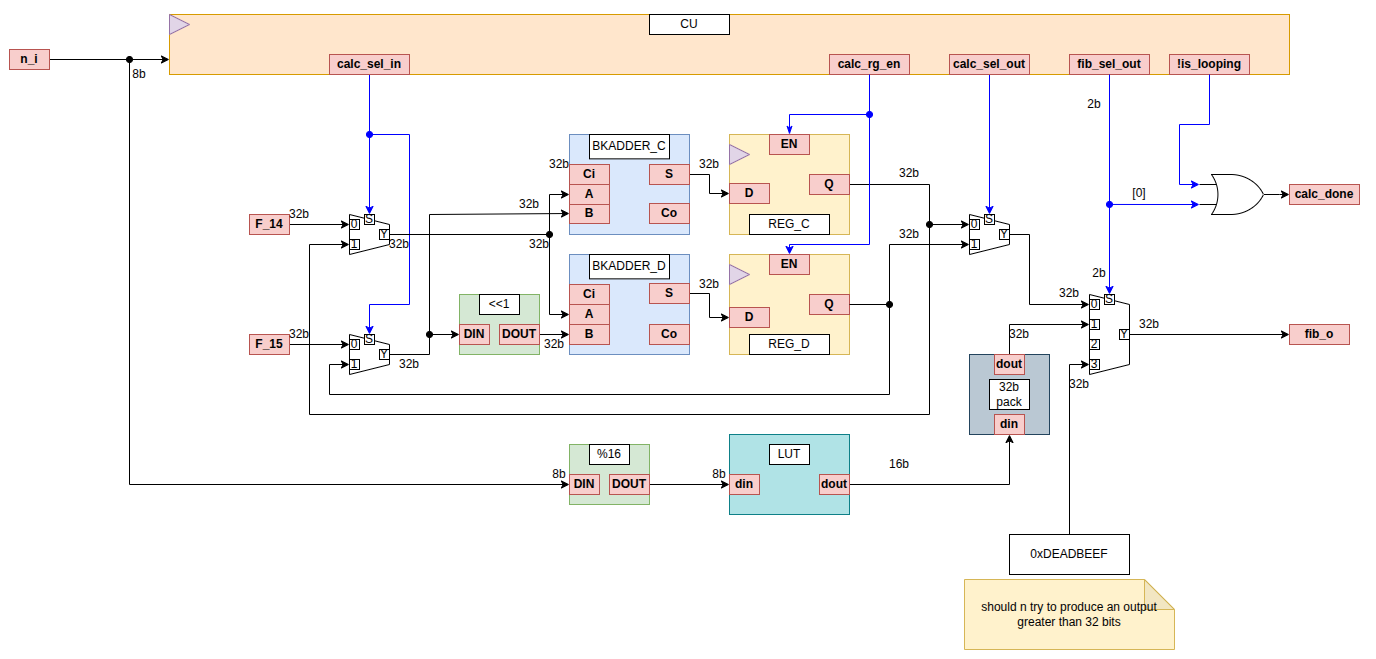
\includegraphics[
				width			= \textwidth,
				keepaspectratio	= true
			]{./pics/accelerator.png}
			\caption{Computation Portion of Fib Accelerator}
			\label{fig:comp}
		\end{figure}

		\begin{figure}[H]
			\centering
			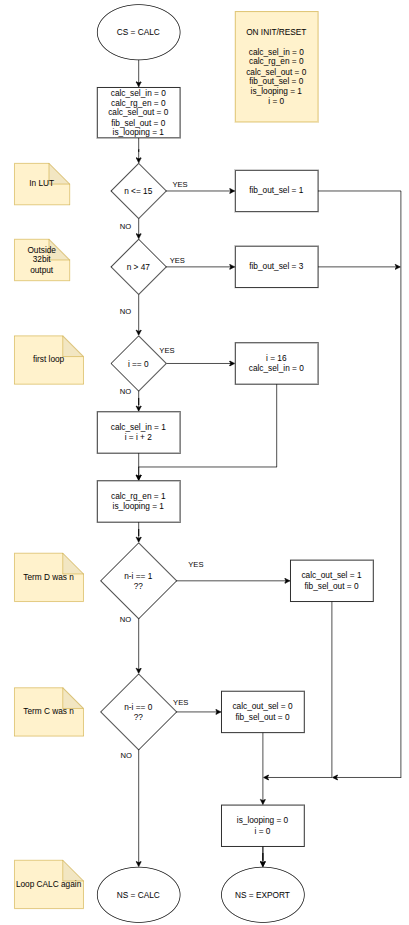
\includegraphics[
				width			= 0.4\textwidth,
				keepaspectratio	= true
			]{./pics/calc_flow.png}
			\caption{Control Flow of CALC State}
			\label{fig:calcflow}
		\end{figure}

		To properly explain the design, let's trace through various values 
		of $n$.

		\begin{figure}[H]
			\centering
			\begin{subfigure}[t][][b]{\textwidth}
				\centering
				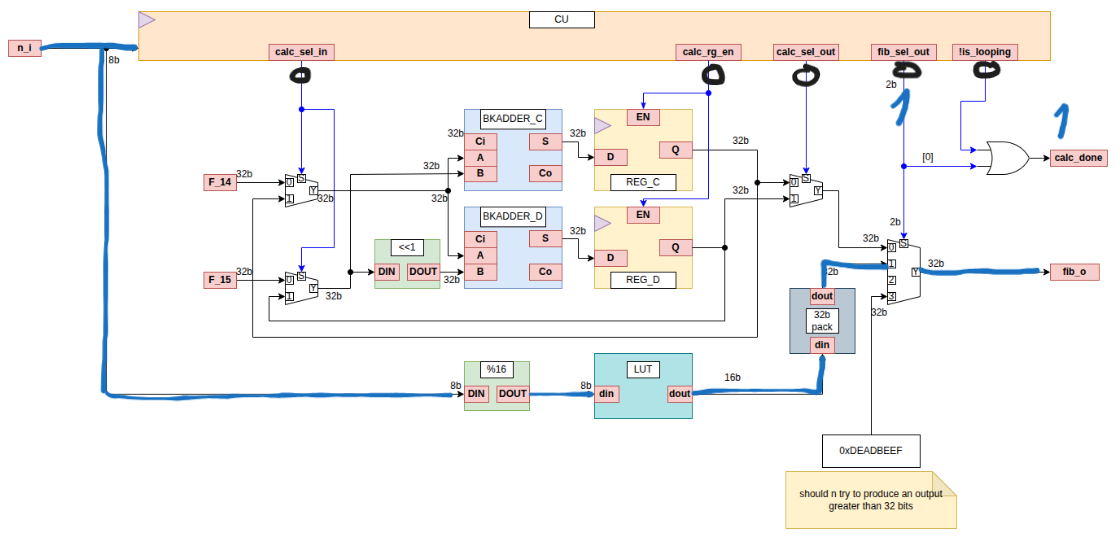
\includegraphics[
					width			= 1.0\textwidth,
					keepaspectratio	= true
				]{./pics/calc_flow_lowLUT.png}
			\end{subfigure}
			\begin{subfigure}[t][][b]{\textwidth}
				\centering
				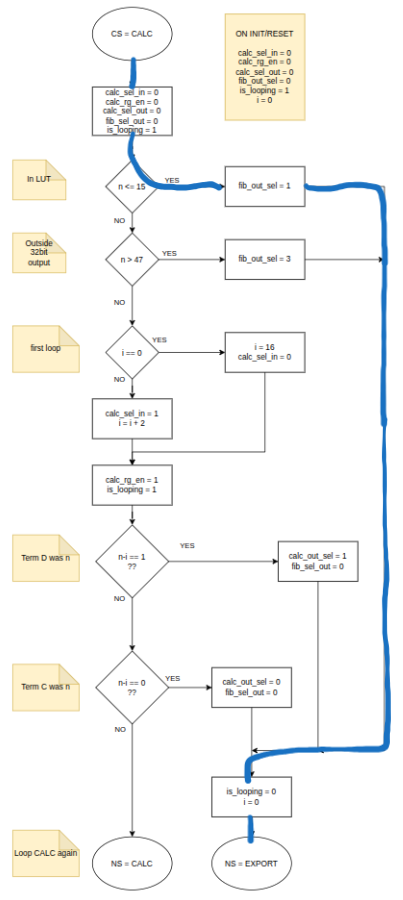
\includegraphics[
					width			= 0.5\textwidth,
					keepaspectratio	= true
				]{./pics/calc_flow_lowLUT1.png}
			\end{subfigure}
			\caption{$n \le 15$ uses the LUT}
			\label{fig:lowlut}
		\end{figure}

		\begin{figure}[H]
			\centering
			\begin{subfigure}[t][][b]{\textwidth}
				\centering
				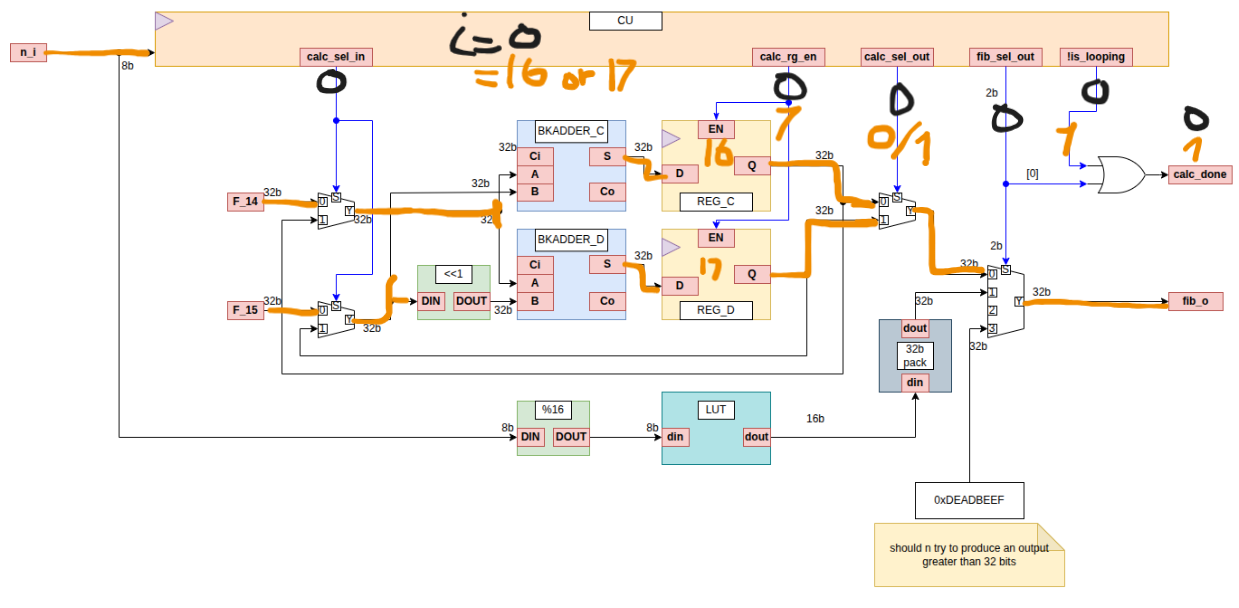
\includegraphics[
					width			= 1.0\textwidth,
					keepaspectratio	= true
				]{./pics/calc_flow_first.png}
			\end{subfigure}
			\begin{subfigure}[t][][b]{\textwidth}
				\centering
				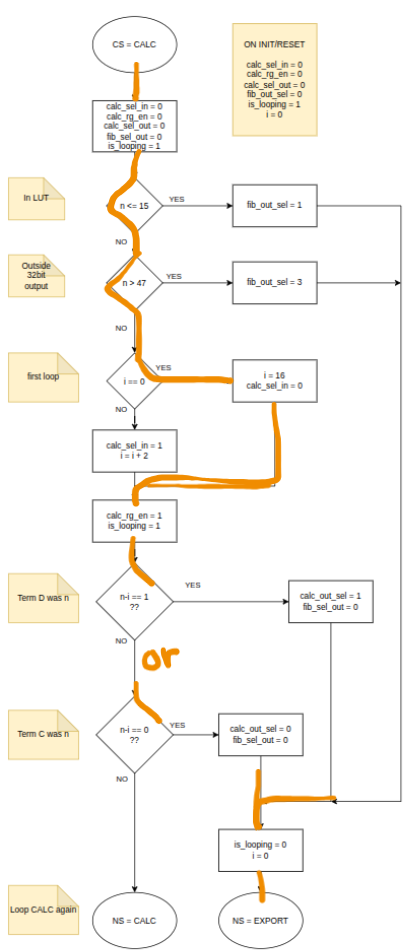
\includegraphics[
					width			= 0.5\textwidth,
					keepaspectratio	= true
				]{./pics/calc_flow_first1.png}
			\end{subfigure}
			\caption{$n = 16$ or $n=17$ calculates but doesn't loop}
			\label{fig:firstcalc}
		\end{figure}

		\begin{figure}[H]
			\centering
			\begin{subfigure}[t][][b]{\textwidth}
				\centering
				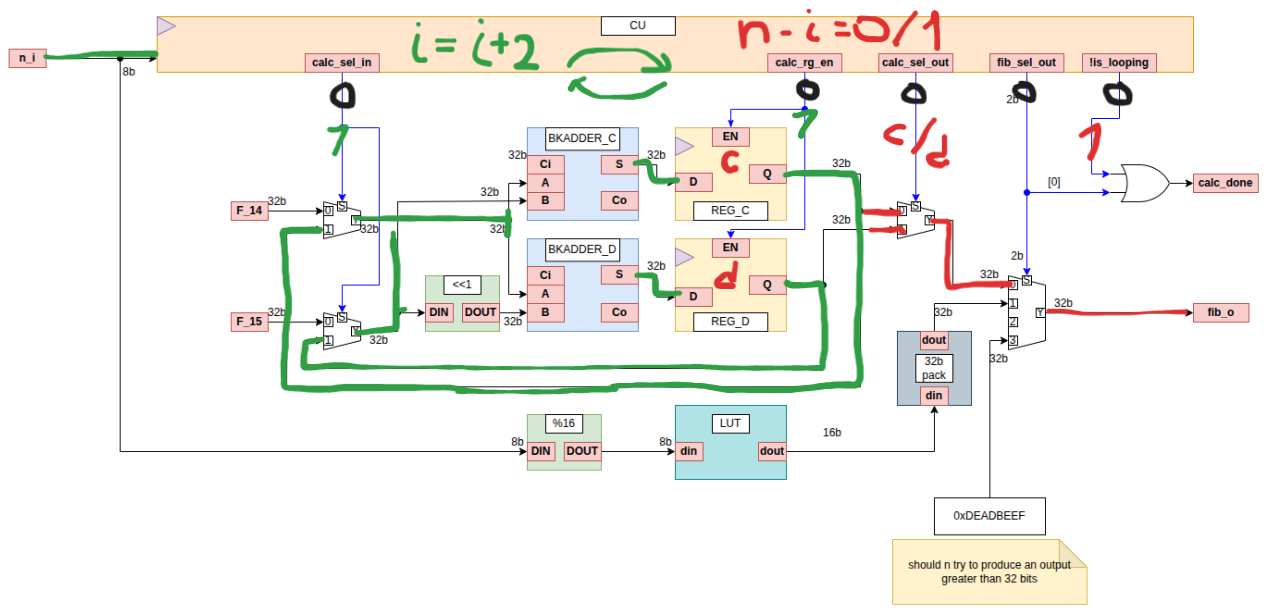
\includegraphics[
					width			= 1.0\textwidth,
					keepaspectratio	= true
				]{./pics/calc_flow_ongoing.png}
			\end{subfigure}
			\begin{subfigure}[t][][b]{\textwidth}
				\centering
				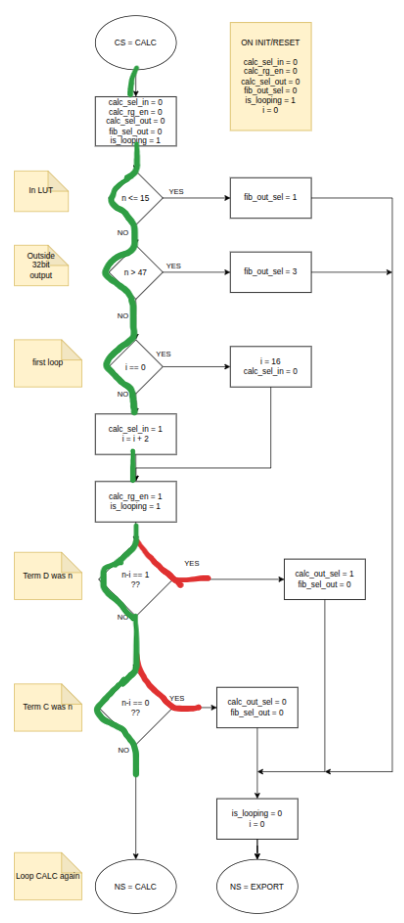
\includegraphics[
					width			= 0.5\textwidth,
					keepaspectratio	= true
				]{./pics/calc_flow_ongoing1.png}
			\end{subfigure}
			\caption{$n \ge 18$ and $n \le 47$ calculates using loops}
			\label{fig:loopcalc}
		\end{figure}

		\begin{figure}[H]
			\centering
			\begin{subfigure}[t][][b]{\textwidth}
				\centering
				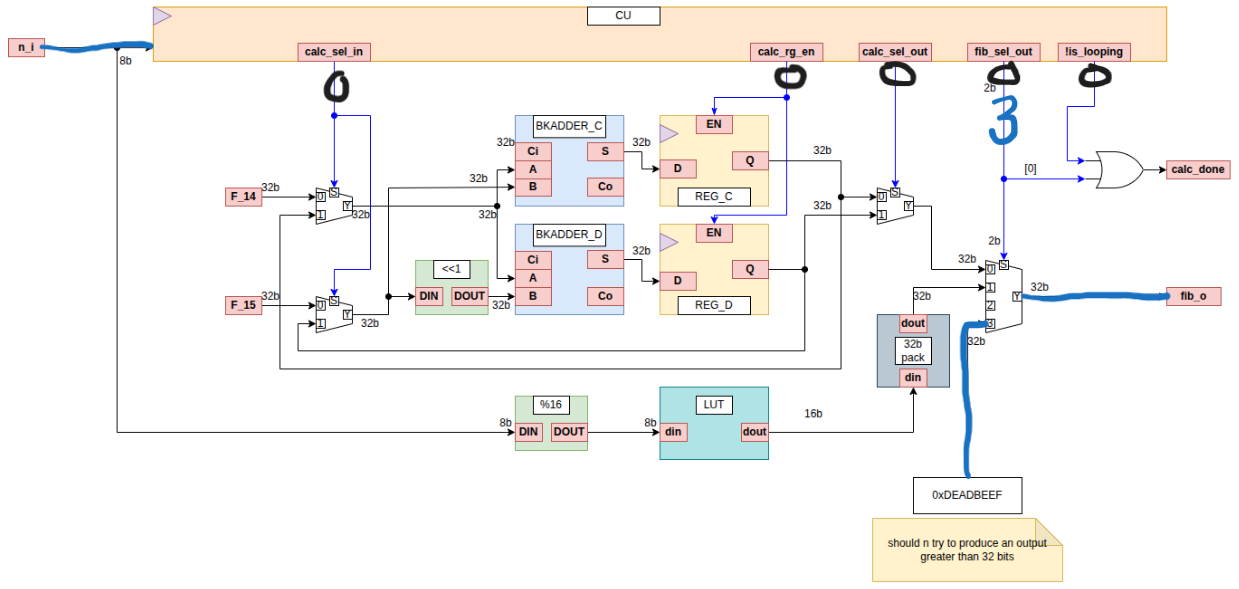
\includegraphics[
					width			= 1.0\textwidth,
					keepaspectratio	= true
				]{./pics/calc_flow_highLUT.png}
			\end{subfigure}
			\begin{subfigure}[t][][b]{\textwidth}
				\centering
				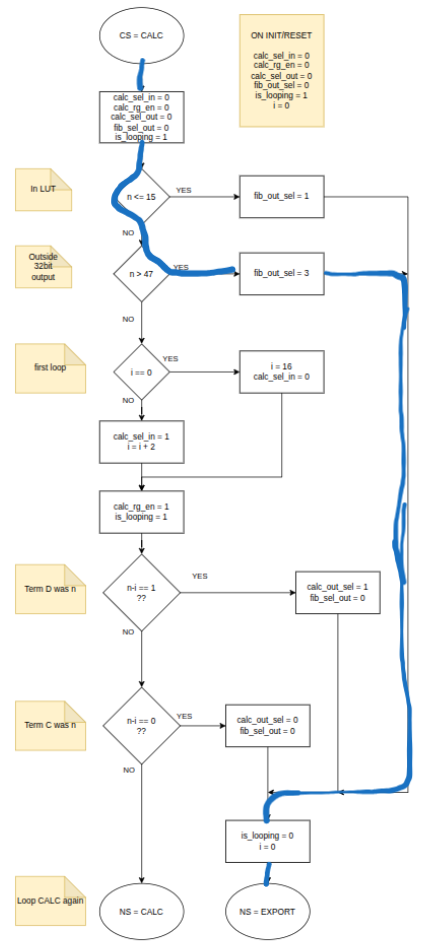
\includegraphics[
					width			= 0.5\textwidth,
					keepaspectratio	= true
				]{./pics/calc_flow_highLUT1.png}
			\end{subfigure}
			\caption{$n > 47$ defaults to avoid output overflow}
			\label{fig:loopcalc}
		\end{figure}

	\chapter{Simulation Testing}

		\section{Brent-Kung `Parallel Prefix' Adder}
			The BKAdder was studied and implemented as a dynamic model, only verified
			using formal verification methods BMC and \textit{K}-Induction. The
			rtl and verification can be seen in the same file~\ref{adder}. 

			\begin{table}[H]
				\centering
				\begin{tabular}{lc}
					\toprule
					\textbf{Test Type} & \textbf{Result} \\
					\midrule
						BMC & \checkmark\\
						\midrule
						Induction & \checkmark\\
					\bottomrule
				\end{tabular}
				\caption{Verification Methods for BKAdder}
			\end{table}

		\section{Fibonacci Accelerator}
			The accelerator was initially verified using immediate and concurrent
			simulations on verilator (not icarus because SVA is not supported). 
			The simulation file~\ref{tb-fib} tests:

			\begin{itemize}
				\item \textbf{Concurrents}
					\begin{itemize}
						\item \textbf{reset\_import}: confirms the module comes out
							of RESET, enters the IMPORT state, and signals the upstream
							that it is ready to accept an input $n$.

						\item \textbf{import\_export}: confirms the model is not 
							holding the output steady while prompting the upstream
							for a new input $n$.

						\item \textbf{hold\_fib}: confirms the output \texttt{fib\_o} was
							steady as long as our module is finished calculating and the downstream
							has not confirmed an output read.
					\end{itemize}

				\item \textbf{Immediates}
					\begin{enumerate}
						\item Test $n \in [0,47]$ outputs the correct values sequentially.
						\item Test $n \in [48,255]$ outputs an error code because output overflow is certain.
					\end{enumerate}
			\end{itemize}

			\begin{table}[H]
				\centering
				\begin{tabular}{lc}
					\toprule
					\textbf{Test Type} & \textbf{Result} \\
					\midrule
						Verilator (SVA) Concurrents & \checkmark\\\midrule
						Verilator (SVA) Immediates& \checkmark\\\midrule
						Icarus (SVA) Immediates& \checkmark\\\midrule
						BMC & \checkmark\\\midrule
						Induction & \XSolidBrush\hl{TODO}\\
					\bottomrule
				\end{tabular}
				\caption{Verification Methods for BKAdder}
			\end{table}

			Overall, the design works well but further verification would make this 
			author feel better about taping on silicon. For now, these desired will be
			placed on hold til the design is viewed with LibreLane. 

	\chapter{Appendix}
		\section{Code}
			\subsection{RTL}
				
				\lstinputlisting[
					language 	= {Verilog},
					captionpos	= top, 
					caption		= {Mux},
					breaklines	= false, 
					label		= {mux}
				]{../rtl/Mux_N.sv}

				\lstinputlisting[
					language 	= {Verilog},
					captionpos	= top, 
					caption		= {Brent-Kung `Parallel Prefix' Adder},
					breaklines	= false, 
					label		= {adder}
				]{../rtl/BKAdder.sv}

				\lstinputlisting[
					language 	= {Verilog},
					captionpos	= top, 
					caption		= {Fibonacci Accelerator},
					breaklines	= false, 
					label		= {fib}
				]{../rtl/fib.sv}

			\subsection{Simulation SVA Testing}

				\lstinputlisting[
					language 	= {Verilog},
					captionpos	= top, 
					caption		= {Testbench simulation for Fibonacci Accelerator},
					breaklines	= false, 
					label		= {tb-fib}
				]{../tests/tb_fib/tb_fib.sv}

		\section{Boneyard}
			\begin{figure}[H]
				\centering
				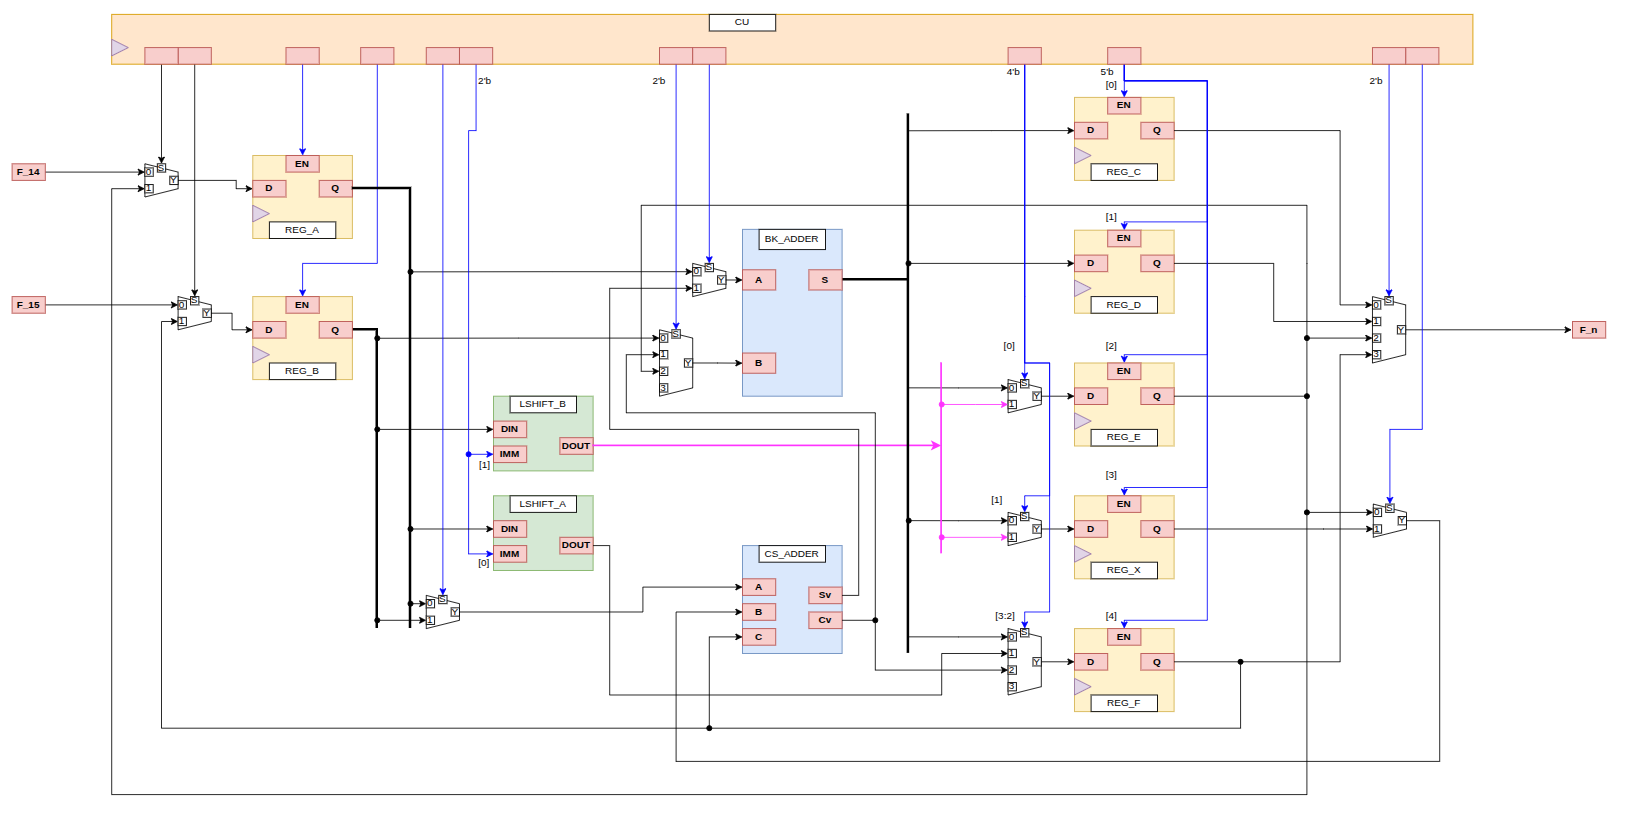
\includegraphics[
					width			= 0.8\textwidth,
					keepaspectratio	= true
				]{./pics/boneyard.png}
				\caption{First Draft of Accelerator}
				\label{fig:boneyard}
			\end{figure}

	\chapter{References}
		\begin{enumerate}
			\item \href{https://github.com/Cal-Poly-Open-Source-ASIC-Class}{CPE490 - OpenSource ASIC}
		\end{enumerate}
		
\end{document}
